\documentclass{article}


% if you need to pass options to natbib, use, e.g.:
%     \PassOptionsToPackage{numbers, compress}{natbib}
% before loading neurips_2022


% ready for submission
% \usepackage{neurips_2022}


% to compile a preprint version, e.g., for submission to arXiv, add add the
% [preprint] option:
%     \usepackage[preprint]{neurips_2022}


% to compile a camera-ready version, add the [final] option, e.g.:
\usepackage[final]{neurips_2022}


% to avoid loading the natbib package, add option nonatbib:
%    \usepackage[nonatbib]{neurips_2022}


\usepackage[utf8]{inputenc} % allow utf-8 input
\usepackage[T1]{fontenc}    % use 8-bit T1 fonts
\usepackage{hyperref}       % hyperlinks
\usepackage{url}            % simple URL typesetting
\usepackage{booktabs}       % professional-quality tables
\usepackage{amsfonts}       % blackboard math symbols
\usepackage{nicefrac}       % compact symbols for 1/2, etc.
\usepackage{microtype}      % microtypography
\usepackage{xcolor}         % colors
\usepackage{color,soul}
\usepackage{hyperref}
\usepackage{graphicx}


\title{Final Project Write-up}


% The \author macro works with any number of authors. There are two commands
% used to separate the names and addresses of multiple authors: \And and \AND.
%
% Using \And between authors leaves it to LaTeX to determine where to break the
% lines. Using \AND forces a line break at that point. So, if LaTeX puts 3 of 4
% authors names on the first line, and the last on the second line, try using
% \AND instead of \And before the third author name.


\author{%
  Caleb Austin and Alex Moree\\
  CSCE 421-500 - Spring 2023\\
  Made with a Template by: Mortazavi
}


\begin{document}


\maketitle


\begin{abstract}
  It is often useful for doctors to be able to predict someone's odds of death when they enter the emergency room, so that they can prioritize care. In this project we are seeking to create an automated system that can take in someone's health information and use that to predict someone's odds of mortality while at the hospital. The consists of some basic information about the patient, such as age and weight, as well information gather about the patient through labs or by the nurse. Each of these different labs or nurse measurements are on different lines connected by a patient id number. Our model combines all the data about each patient into a single data point and builds gradient boosted trees to predict the patient's odds of mortality. Our results with this model have been good; we got more than 92\% accuracy on our testing data. 
\end{abstract}


\section{Introduction}

In this project we were seeking to create a model that would provide medical professionals with a way of accurately determining the odds that any given emergency room patient would survive their hospital stay. This allows them to give more attention to those who are mostly likely to die, so as to minimize deaths. To build our model we chose to use gradient boosted trees. We originally used an RNN, but only got mediocre results; so we tried to use gradient boosted trees, because they tend to provide good results on large datasets with a lot of features. We have since gotten good results. Specifically, we got more than 92\% accuracy on our test dataset. 

\section{Your Method}

For our model we first compressed each patient's health records into a single data point. Then, we build gradient boosted trees using those data points. Those trees can now be used to predict the mortality of anyone who's health records have been put in the same format. 

\subsection{Data Preprocessing}

For preprocessing our model first converts the \texttt{patientunitstayid} to an integer to avoid issues when working with it. Then, we drop any data points with the \texttt{nursingchartvalue} of \texttt{Unable to score due to medication}; those data points won't work within the model and don't have much information anyway. Next, we convert all the \texttt{nursingchartvalue} to floats (or NaN if they cannot be converted) so that they can be processed as numbers (without lossing all the data contained in data points without this feature). We create a copy of the original dataset with the \texttt{admissionheight}, \texttt{admissionweight}, \texttt{age}, \texttt{gender}, \texttt{patientunitstayid}, and \texttt{unitvisitnumber}. This copy is what we will ultimately use with the model. Creating a copy is not necessary, but simplifies the process of preprocessing the data by allowing us to build the data from the ground up rather than having to modify an already existing dataset. After creating the copy, we one-hot encode the gender feature and replace \texttt{> 89} with 100 in the age column. This prevents issues with cases where the gender feature isn't filled in and makes sure the age column is always a number so that \texttt{> 89} cannot create an error. Next, we drop duplicates in the \texttt{patientunitstayid} column and make the \texttt{patientunitstayid} column the index. This makes it so that each patient is just one data point to simplify the model and make it so that data on a patient is indexed by their id. 

After that, we proceed to create data columns, copy other pieces of the original dataset and modify them in minor ways, before pulling the data out of them and putting it into our first copy. For the first round of this, we create a data column in first copy called \texttt{cellattributevalue} and set it to \texttt{None}. This provides us a place to fill in those values, and will have a default value if there is nothing. We create a second copy of the dataset with the \texttt{cellattributevalue}, \texttt{celllabel}, \texttt{offset}, and \texttt{patientunitstayid}. We drop any data points in that copy with missing values to keep the data clean. Then, we encoded \texttt{< 2 seconds}, \texttt{> 2 seconds}, \texttt{normal}, \texttt{hands}, and \texttt{feet} as numbers to make it easier for the model to work with them. After that, we copied that value into the \texttt{cellattributevalue} feature in the data point in the first copy with the same patient id. For the second round, we create \texttt{pH} and \texttt{glucose} columns and fill them with \texttt{None}. Then, we create a third copy of the dataset with the \texttt{labname}, \texttt{labresult}, \texttt{offset}, and \texttt{patientunitstayid} features. Next, we drop any data point with missing values in the third copy. After that, we copy the \texttt{labresult} into the \texttt{labname} feature in the data point with the same patient id in the first copy. If there is already some number in the \texttt{labname} feature, the smaller value is used. For the final round, we add the columns \texttt{GCS Total}, \texttt{Heart Rate}, \texttt{Non-Invasive BP Diastolic}, \texttt{Non-Invasive BP Mean}, \texttt{Non-Invasive BP Systolic}, \texttt{Invasive BP Diastolic}, \texttt{Invasive BP Mean}, \texttt{Invasive BP Systolic}, \texttt{Respiratory Rate}, and \texttt{O2 Saturation} and fill them with \texttt{None}. Then, we create a fourth copy of the dataset with the \texttt{nursingchartcelltypevalname}, \texttt{nursingchartvalue}, \texttt{offset}, and \texttt{patientunitstayid}. Next, we drop any data points that contain any missing values. After that, we copy the \texttt{nursingchartvalue} in the \texttt{nursingchartcelltypevalname} feature in the data point in the first copy with the same patient id, unless the is already a smaller value there. 

Finally, we convert all the data into floats and fill in any missing values with the average value for that feature. This prevents any errors from missing values or values being an unexpected type. 

\subsection{Model Design}

Our model consists of a set of gradient boosted trees. We choose to use gradient boosted trees, because they tend to work well on large datasets with lots of features. In particular we used sklearn's GradientBoostingRegressor with 600 boosting stages. The trees generated during each of these stages were limited to a depth of 2, each leaf had to have at least 4 samples, and any internal node could not be split unless at least 2 samples reached it. We used at learning rate of 0.01 and a random seed of 42. These hyperparameters were originally derived from hyperparameter tuning; except the random seed, because that is random. We subsequently performed some manual testing to find some slightly better hyperparameters. 

\subsection{Model Training}

We simply used sklearn's fit method to train our model. Internally, that works by first selecting the average of the expect value. Then, for each of the 600 boosting stages, it adds the set of trees with a new tree conformant to the parameters given above. Each new tree selected to minimize the loss function, mean-squared error in this case. However, each new tree is only optimized on a random half of the data. Only training each tree on half of the data prevents overfitting. 

\subsection{Hyperparameter Tuning}

We conducted hyperparameter tuning using sklearn's GridSearchCV. GridSearchCV takes in the GradientBoostingRegressor model and a dictionary defining the hyperparameters we want it to test. We had it conduct 5-fold cross validation on every possible combination of the hyperparameter we gave to it. We had it try 400, 500, 600, or 700 boosting stages; a learning rate of 0.1, 0.01, or 0.001; a maximum tree depth of 3, 4, or 5; and subsample sizes of 0.25, 0.5, or 0.75 for building each tree. 

\section{Results}

The results of our model have been quite good. To demonstrate we preprocessed our data as before and split off 20\% of the data to be validation data. We trained numerous different models on the training data and tested it on the validation data using four different metrics. 
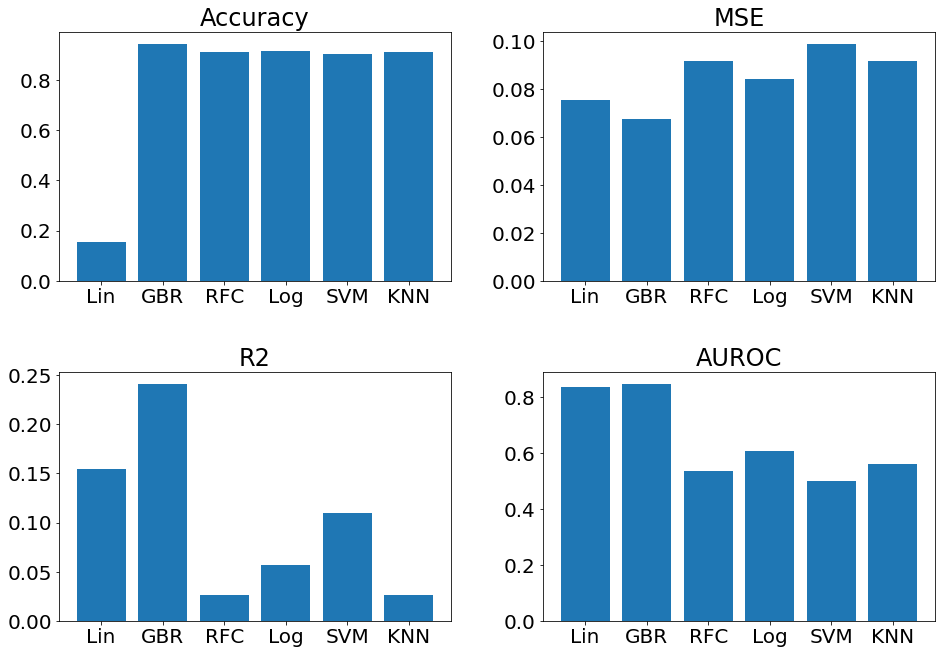
\includegraphics[width=\linewidth]{FinalResults.png}
We abbreviated the names of the different models to make them easier to read. You can use the table below if you are unsure as to what any model is. 

\begin{tabular}{|c|c|}
    \hline
    Abbreviation & Model\\
    \hline
    Lin & Linear Regression\\
    GBR & Gradient Boosting Regressor\\
    RFC & Random Forest Classifier\\
    Log & Logistic Regression\\
    SVM & Support Vector Machine\\
    KNN & k-Nearest Neighbors\\
    \hline
\end{tabular}

As you can see our model preformed best on every metric except mean squared error. It achieved more than 92\% accuracy on the hidden test data. 

\section{Conclusion}

The hardest part of this project was explicitly the processing of the dataset and subsets. This took a lot of online searching and out-of-the-box thinking that one would normally oversee to create the end result. We think some of the difficulty was due to our unfamiliarity with medical data. If we where more accustomed to this type of data this process would have been simpler. Splitting the data into subsamples was by far the most effective strategy for improving accuracy. Then, we just needed to find a model competent with large numbers of features which was why we chose Gradient Boosting. It was actually by accident, as the first option was XGBoost, but we encountered import errors, so we tried the Random Forest Classifier, but it overfit the data way too much and resulted in low accuracy scores. Lastly Gradient Boost was chosen, because it was referenced in some of the lecture material and we decided to give it a shot. This endeavor proved to be quite fruitful. Gradient Boost is good for large feature sets because it can handle high-dimensional data and feature interactions, leading to better predictive accuracy resulting in what you see now. 


\end{document}
